\documentclass{article}
\usepackage[a4paper, top=2.5cm, bottom=2.5cm, left=2.5cm, right=2.5cm]{geometry}
\usepackage[utf8]{inputenc}
\usepackage[T1]{fontenc}
\usepackage{indentfirst}
\usepackage{tabularx}
\usepackage{graphicx}
\usepackage{color}
\usepackage{amsmath}
\usepackage{amssymb}
\usepackage{titling}
\usepackage{float}
\usepackage{geometry}
\newcommand{\ii}{\textit}


\title{Impact of network topology on opinion dynamics in a Bounded Confidence model}
\author{Artur Przybyłek}

\begin{document}

\begin{titlepage}
	\maketitle
	\begin{abstract}
	In this paper we will investigate impact of network topology on proccess of spreading opinions in Bounded Confidence model. We will conduct Monte Carlo simulations on various model and real networks and various variants of Bounded Confidence model.
	\end{abstract}
\end{titlepage}


\tableofcontents

\newpage

\section{Introduction}
% \section{Modelling opinions dynamics}
\section{Bounded Confidence model}
	
\subsection{Symmetric confidence level}
\subsection{Opinion--dependent confidence level}
%\subsection{Agent--dependent confidence level}

\section{Simulations}

\subsection{Simulations methodology}

We will perform simulations of the bounded confidence model on various underlying network topologies:
\begin{itemize}
\item complete graph
\item Watts--Strogatz graph
\item Barabasi--Albert graph
\end{itemize}
Througout this section we will use some common names for network parameters:
\begin{itemize}
\item $n$: size of the network
\item $k$: mean degree in Watts--Strogatz graph
\item $p$: probability of changing edge in creation of Watts--Strogatz graph
\item $m$: number of new connections for each node in creation of Barabasi--Albert graph
\end{itemize}
Changing parameters both of the model and the network, we will study such features as:
\begin{itemize}
\item impact of confidence level for reaching consensus
\item distribution of final opinions
\item opinions changes through simulation
\item fragmentation of opinions
\end{itemize}

For each simulation of the model we will start with new instance of underlying network and set of random agent opinions with uniform distribution $\mathcal{U}(0, 1)$. Then, in each step we will $n$--times randomly choose an agent and change his opinion by applying bounded confidence model rule. We will consider simulation as finished when none of the agents will change his opinion by more than 0.001 in one simulation step. 
\indent

We will conduct simulations on the machine with dual--core 1.8 GHz processor: AMD E2-3000M APU. We will use Python 3.6.4 programming language.

\subsection{Single simulations of the model}
In order to see how opinions changes through time, we will plot agents opinions against time for several single simulations of Bounded Confidence model. We will do this for 4 different values of confidence level: $\epsilon=0.05, 0.15, 0.25, 0.35$ using different underlying network topologies.

\subsubsection{Complete graph}

\begin{figure}[H]
		\centering
		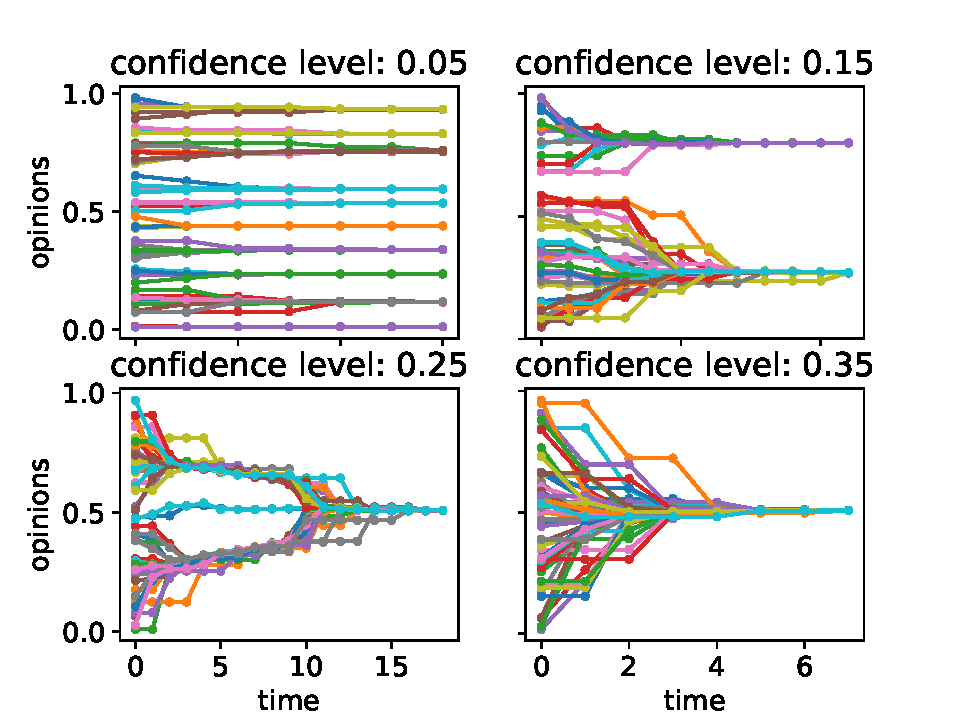
\includegraphics[width=\textwidth]{/home/arti/studia/python/praca_magisterska/plots/single_cg_50.pdf}
		\caption{Opinions dynamics for complete graph network with $n=50$}
\end{figure}
As we can see on the above figure for higher values of confidence level ($0.25, 0.35$) agents reach consensus at the end of simulation. For small confidence level ($0.05$) there occurs fragmentarization of opinions -- 11 clusters are formed and for confidence level $\epsilon=0.15$ opinions dynamics leads to fragmentarization of 3 clusters.
\indent

In most cases biggest changes of opinions occur in early phase of opinion dynamics but we can see that for confidence level $\epsilon=0.25$ in first phase two big clusters were formed and one small between them and in second phase clusters merged in one. We will investigate when agents change their opinions the most more accurately later on. For $\epsilon=0.35$ also consensus was reached.

\subsubsection{Watts--Strogatz}

\begin{figure}[H]
		\centering
		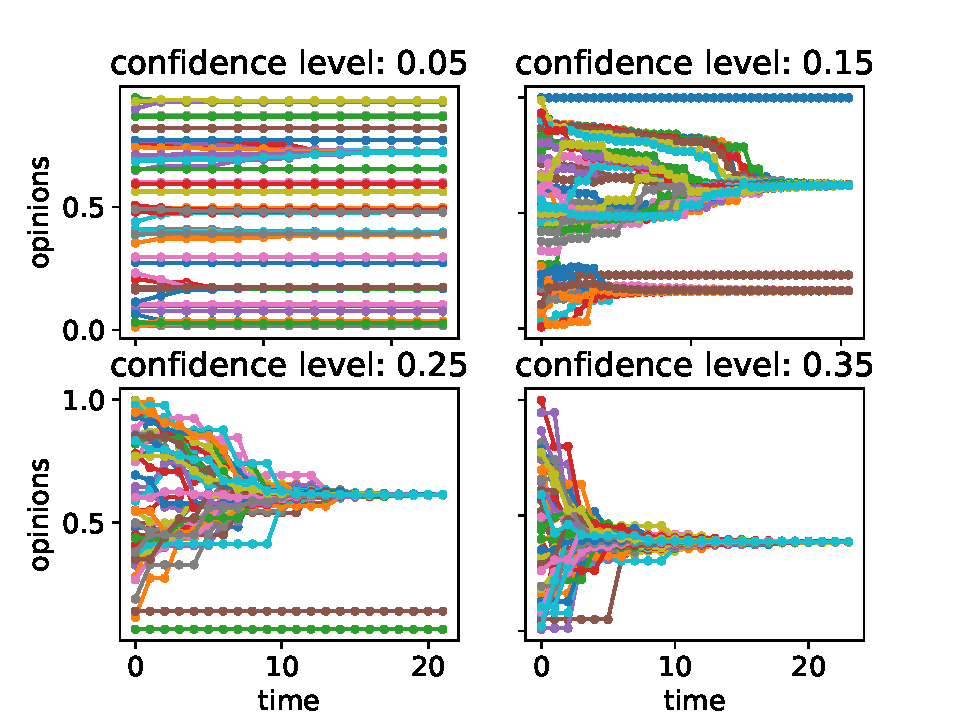
\includegraphics[width=\textwidth]{/home/arti/studia/python/praca_magisterska/plots/single_ws_50_10_0,3.pdf}
		\caption{Opinions dynamics for Watts--Strogatz network with $n=50$, $k=10$, $p=0.3$}
\end{figure}
For Watts--Strogatz networks we can observe that for confidence level $\epsilon=0.05$ fragmentarization of opinions also occurs but this time much more clusters are formed, which is caused by smaller number of connections, agents can not influence another ones if they do not know each other (even if their opinions are similiar). 
\indent

For confidence level $\epsilon=0.15$ opinions evolution leaded to formation of 3 clusters. For confidence level $\epsilon=0.25$ most part of network reached consensus, excluding two agents who didn't change their initial opinions at all, in fact their opinions are extreme ones (close to 0 or 1). Interestingly, when confidence level was big enough ($\epsilon=0.35$) all agents in network decided to share one opinion.
\indent

Relaxation time of opinions formation is longer than for complete graph network, especially for $\epsilon=0.15$ agents change their opinions very slowly.

\subsubsection{Barabasi--Albert}

\begin{figure}[H]
		\centering
		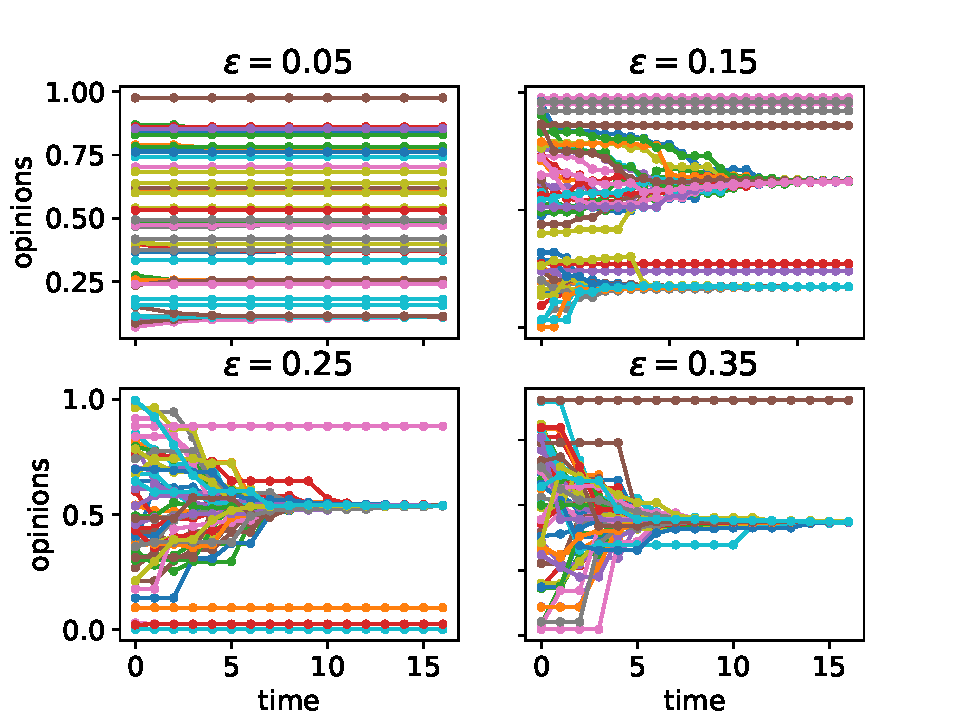
\includegraphics[width=\textwidth]{/home/arti/studia/python/praca_magisterska/plots/single_ba_50_4.pdf}
		\caption{Opinions dynamics for Barabasi--Albert network with $n=50$, $m=4$}
\end{figure}
In the case of Barabasi--Albert network we see that agents change their opinions mostly in the first phase of opinions dynamics. Due to small number of connections we have some agents who don't change their opinions for every considered consensus level. Usually their opinions are extreme ones. Excluding these non--influencial individuals, we may state that consensus was reached for $\epsilon=0.25, 0.35$.

\subsection{Final opinions distribution}

We will now investigate what is typical distribution of opinions in network depending on value of confidence level. We rounded final opinions of agents to two decimal places and calculated average frequency of opinions occurences. We present the results on three--dimensional plots. One dimension represents opinion space, second confidence level and third one is opinion frequency.

\subsubsection{Complete graph}

\begin{figure}[H]
		\centering
		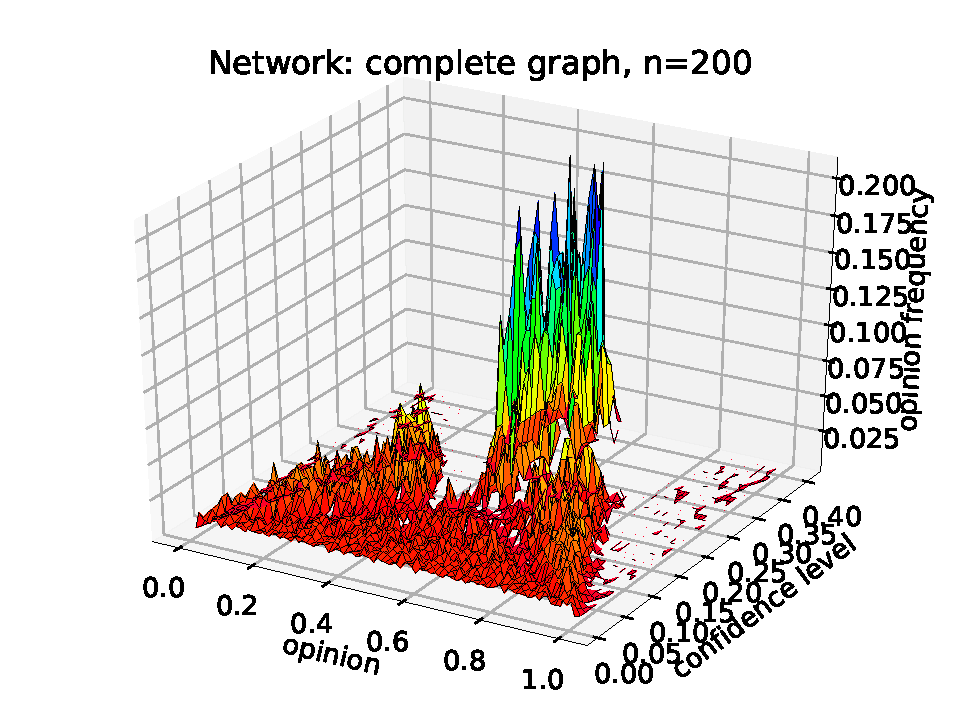
\includegraphics[width=\textwidth]{/home/arti/studia/python/praca_magisterska/plots/avg_freq_cg_200.pdf}
		\caption{Average frequency of final opinions for complete graph network with $n=200$}
\end{figure}

For complete graph we obtained similiar results as in (Hegselmann and Krause 2002), however we have some agents with different opinions even if most of the network reach consensus ($\epsilon > 0.25$), it is caused by different updating schema, in our case there is non--zero probability that agent's opinion will be not influenced for some time and that in the same time other agents will change their opinions strongly enough to break confidence between them.
\indent

Looking closer to average frequency of final opinions for complete graph, we can see that as the confidence level grows, the distribution of opinions is more centralised. For very small confidence level ($\epsilon=0.01$) opinions are distributed uniformly on interval $(0, 1)$ (fragmentarization). As confidence level increases, opinions distribution changes. When we look at confidence level $\epsilon=0.1$ we can observe similiar distribution in the middle of opinion space ($0.25-0.75$) but extreme opinions (close to 0 or 1) do not emerge and opinions in spaces $0.1-0.25$ and $0.75-0.9$ appear more frequently. This phenomena of disappearance of extreme opinions and more frequent appearance of opinions in two regions which are symmetric with respect to the middle of opinions space continues to evolve up to confidence level $\epsilon=0.2$. We can also see that as we are closer to confidence level $\epsilon=0.2$, in the middle of opinions space ($0.35-0.65$) less opinions survive, this is a typical case of polarization of opinions.
\indent

If we increase confidence level again to $\epsilon=0.25$ we can observe changing from polarization of opinions to reaching consensus. In case of consensus final agents opinions concentrate around the middle of opinion space ($0.5$).


\subsubsection{Watts--Strogatz}

\begin{figure}[H]
		\centering
		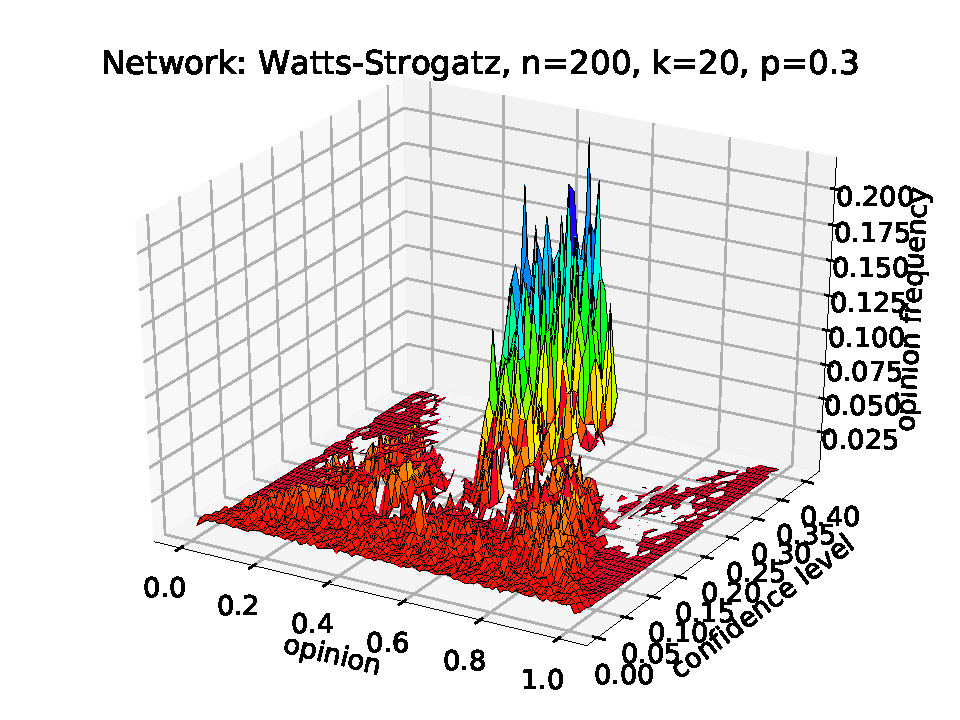
\includegraphics[width=\textwidth]{/home/arti/studia/python/praca_magisterska/plots/avg_freq_ws_200_20_0,3.pdf}
		\caption{Average frequency of final opinions for Watts--Strogatz network with $n=200$, $k=20$, $p=0.3$}
\end{figure}

Average frequency of final opinions for Watts--Strogatz network looks similiar to complete graph case but there are some differences worth mention. We can observe that for small confidence levels ($\epsilon<0.15$) extreme opinions still occur and these are rather single cases, because their frequency is close to 0. For confidence level $\epsilon=0.2$ distribution of opinions is also polarized and then for bigger confidence levels consensus is reached but still sometimes single extreme opinions survive.

\subsubsection{Barabasi--Albert}

\begin{figure}[H]
		\centering
		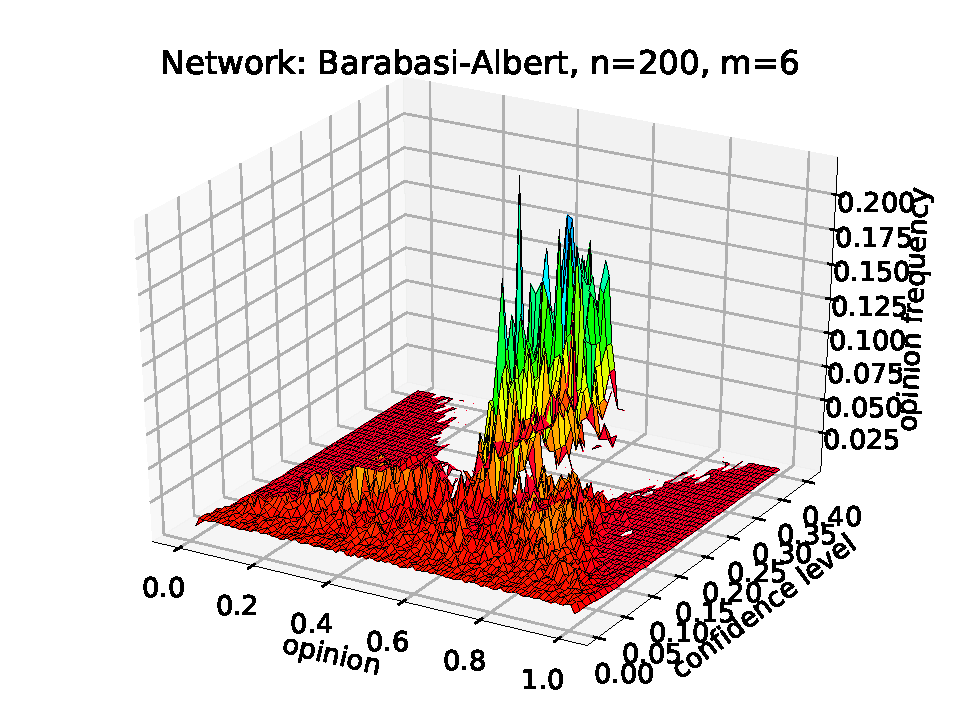
\includegraphics[width=\textwidth]{/home/arti/studia/python/praca_magisterska/plots/avg_freq_ba_200_6.pdf}
		\caption{Average frequency of final opinions for Barabasi--Albert network with $n=200$, $m=6$}
\end{figure}

For Barabasi--Albert case extreme opinions survive the most frequently, the polarization of opinions for confidence level $\epsilon=0.2$ is not so well visible, in fact at this level it seems that network starts to reach consensus. Of course, the results might be little different when network will have more connections (bigger value of parameter $m$), we will investigate this in following sections.

\subsection{Impact of confidence level for reaching consensus}
We will investigate in this section which values of confidence level typically lead to consensus as final state of model evolution and how does the network size and network topology parameters affect frequency of reaching consensus. For each network topology we conduct simulations for various sets of parameters. We assume that consensus is reached when 80\% of agents share common opinion. For each value of confidence level and given network topology with its parameters, we simulate bounded confidence model 100 times and calculate frequency of reaching consensus as a final state. To present our results, we will plot frequency of reaching consensus against confidence level.

\subsubsection{Complete graph}
The following figure shows the impact of network size on frequency of reaching consensus for complete graph topology.
\begin{figure}[H]
		\centering
		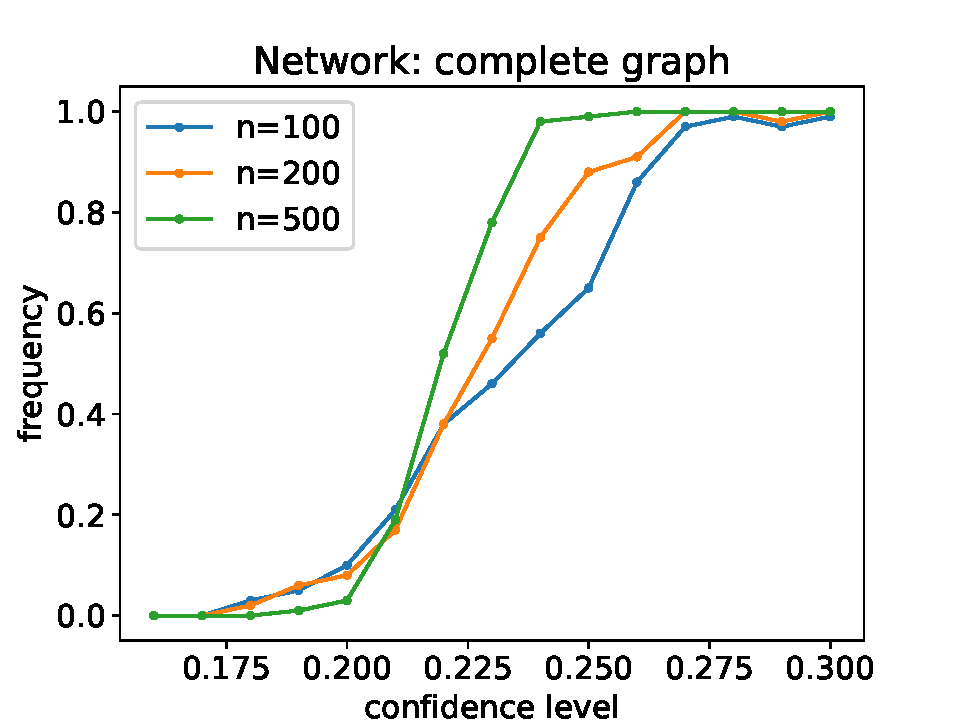
\includegraphics[width=\textwidth]{/home/arti/studia/python/praca_magisterska/plots/freq_consensus_cg.pdf}
		\caption{Frequency of reaching consensus for complete graph network}
\end{figure}

We observe that for confidence level $\epsilon<0.21$ smaller networks are more likely to reach consensus state, while for $\epsilon>0.21$ bigger networks are more likely to reach consensus state. 
\indent

For networks of sizes $n=100$, $n=200$ when confidence level $epsilon\leq0.18$ we hardly ever reach consensus, while $epsilon\geq0.27$ leads to reaching consensus almost every time.
For network size $n=500$ we hardly ever reach consensus when $\epsilon\leq0.2$ and almost every time reach censensus when $\epsilon\geq0.24$. The difference between these critical confidence levels is in this case much smaller, which suggests that when network size $n \to \infty$ there might be critical confidence level such that for smaller level consensus is unlikely to be reached and for bigger level consensus is almost sure to be reached. 

\subsubsection{Watts--Strogatz}

Firstly we set Watts-Strogatz network parameters $k=30, p=0.3$ and by manipulating network size, we conduct simulations of a model.

\begin{figure}[H]
		\centering
		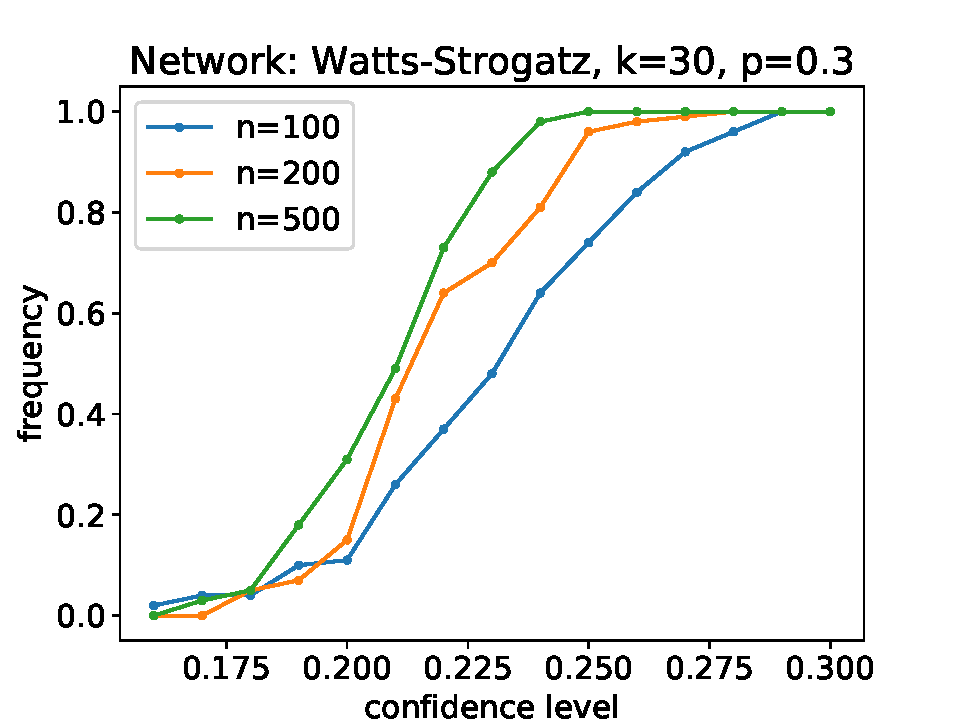
\includegraphics[width=\textwidth]{/home/arti/studia/python/praca_magisterska/plots/freq_consensus_ws_k=30_p=0,3.pdf}
		\caption{Frequency of reaching consensus for Watts--Strogatz network with $k=30, p=0.3$}
\end{figure}

We can see on the above figure that the bigger value of network size is, we obtain frequency of reaching consensus close to 1 for smaller values of confidence level. For instance we reach consensus almost every time at confidence level:
\begin{itemize}
\item  $\epsilon=0.29$ for network size $n=100$,
\item  $\epsilon=0.26$ for network size $n=200$,
\item  $\epsilon=0.24$ for network size $n=500$.
\end{itemize}
\indent

Next, we will check what influence on reaching consensus does manipulating parameter $k$ has. For that purpose we set network size $n=200$, parameter $p=0.3$ and conduct simulations. We plot obtained results and also results for complete graph for comparison.

\begin{figure}[H]
		\centering
		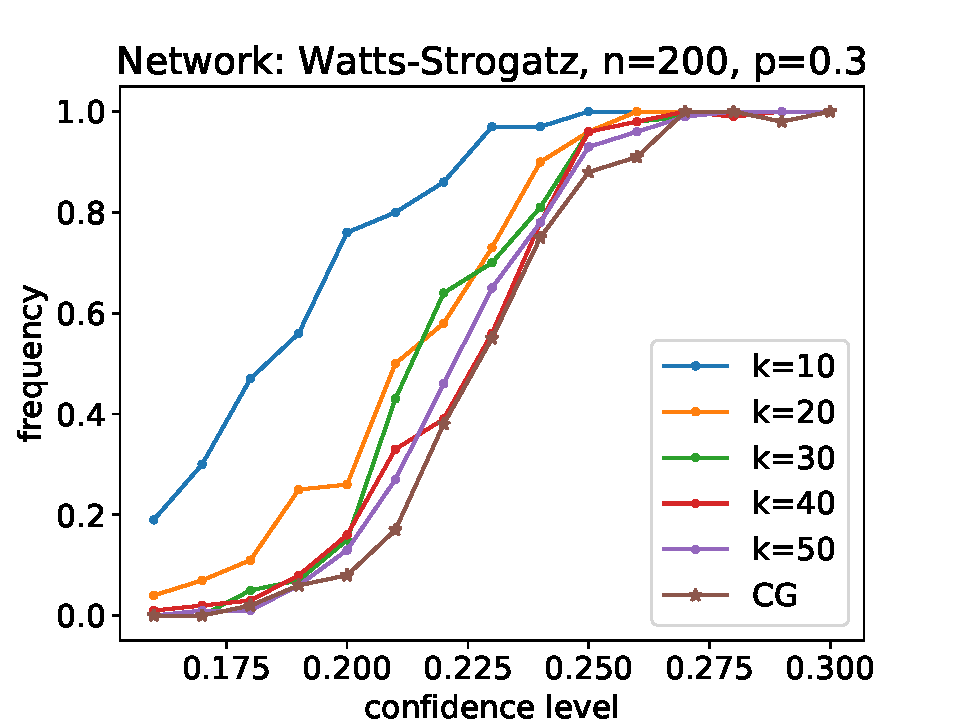
\includegraphics[width=\textwidth]{/home/arti/studia/python/praca_magisterska/plots/freq_consensus_ws_200_p=0,3.pdf}
		\caption{Frequency of reaching consensus for Watts--Strogatz network with $n=200, p=0.3$}
\end{figure}

We can see that the bigger parameter $k$ is, the less often we are reaching consensus. It means that for Watts-Strogatz network if average number of agent connections is small, it is more likely that consensus will establish, than if network is well--connected. For instance, we obtained consensus in 80\% of simulations for confidence level $\epsilon=0.2$ when $k=10$ and not even in 30\% of simulations for $k\geq20$.
\indent
Moreover, we see that plot for complete graph (labeled CG) is the right--most in the figure, which implies that for fully--connected network it is harder to reach consensus. For confidence level $\epsilon\geq0.26$ we almost every time reach consensus for every considered network.

\indent


To better understand what $k$ values are typical for reaching consensus, we also plot frequency of reaching consensus against $k$ in range $(4-20)$ for few values of confidence level.

\begin{figure}[H]
		\centering
		\includegraphics[width=\textwidth]{/home/arti/studia/python/praca_magisterska/plots/eps_freq_consensus_ws_200_p=0,2.pdf}
		\caption{Frequency of reaching consensus in terms of $k$ parameter of Watts--Strogatz network}
\end{figure}

It turns out that consensus is most likely to be reached when $k=6$ and $k=8$, which are cases of low number of connections. For $k=4$ agents are too weekly--connected and they can not influence each other so much, thus they agree on consensus rarely. For $\epsilon$ up to $0.22$ increasing $k$ starting from $k=8$ causes decreasing of frequency of reaching consensus.

\indent

We already manipulated $n$ and $k$ parameters, now we will simulate model for different values of parameter $p$, setting $n=200$, $k=20$.

\begin{figure}[H]
		\centering
		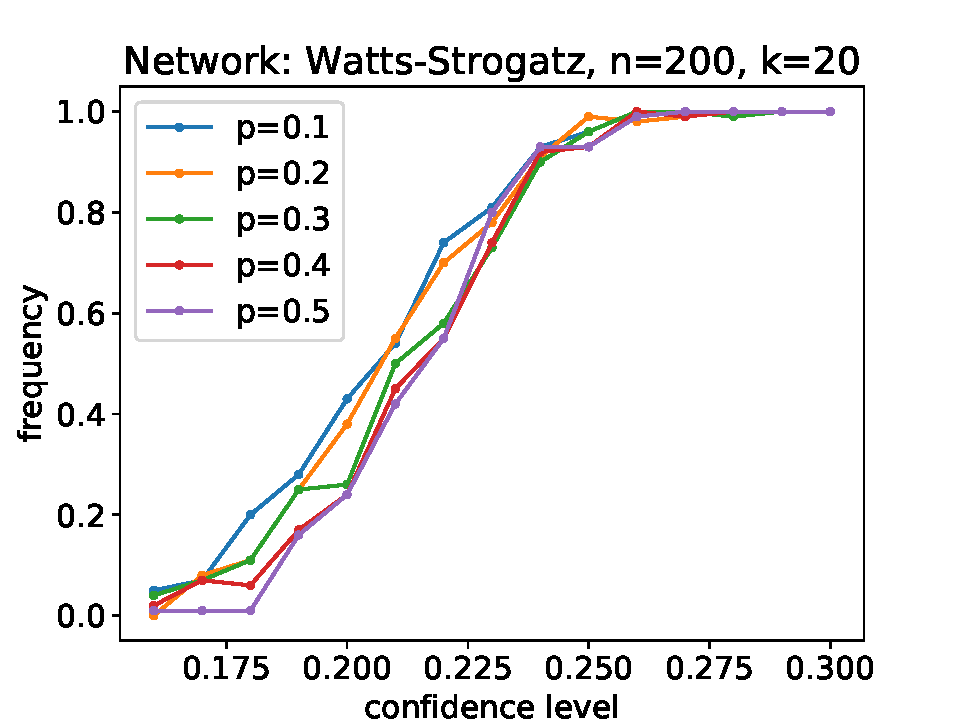
\includegraphics[width=\textwidth]{/home/arti/studia/python/praca_magisterska/plots/freq_consensus_ws_200_k=20.pdf}
		\caption{Frequency of reaching consensus for Watts--Strogatz network with $n=200, k=20$}
\end{figure}

We can see that plot for the smallest considered value $p=0.1$ is the left--most, while for biggest considered value $p=0.5$ is the right--most. In this case differences between the plots are not as big as in the case of manipulating parameter $k$, but still we can observe that the bigger value of parameter $p$ is, the less likely is the network to achieve consensus state.

\subsubsection{Barabasi--Albert}

For Barabasi--Albert network topology firstly we set $m=6$ and manipulate network size $n$.

\begin{figure}[H]
		\centering
		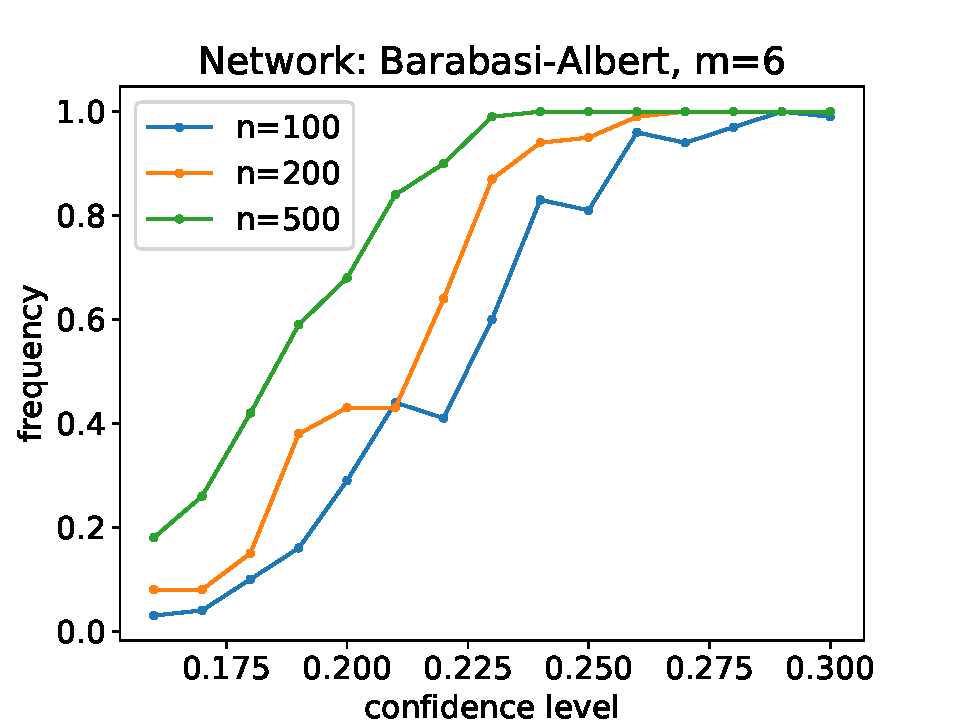
\includegraphics[width=\textwidth]{/home/arti/studia/python/praca_magisterska/plots/freq_consensus_ba_m=6.pdf}
		\caption{Frequency of reaching consensus for Barabasi--Albert network with $m=6$}
\end{figure}

Similary to the case of Watts--Strogatz network topology, increasing network size in Barabasi--Albert case also affects more frequent reaching consensus state for given confidence level. Frequency of reaching consensus is close to 1, when:
\begin{itemize}
\item  $\epsilon=0.29$ for network size $n=100$,
\item  $\epsilon=0.26$ for network size $n=200$,
\item  $\epsilon=0.22$ for network size $n=500$.
\end{itemize}
\indent

Next, we manipulate parameter $m$, setting $n=200$, simulate and plot results. We also plot results for complete graph (CG) for purpose of comparison.

\begin{figure}[H]
		\centering
		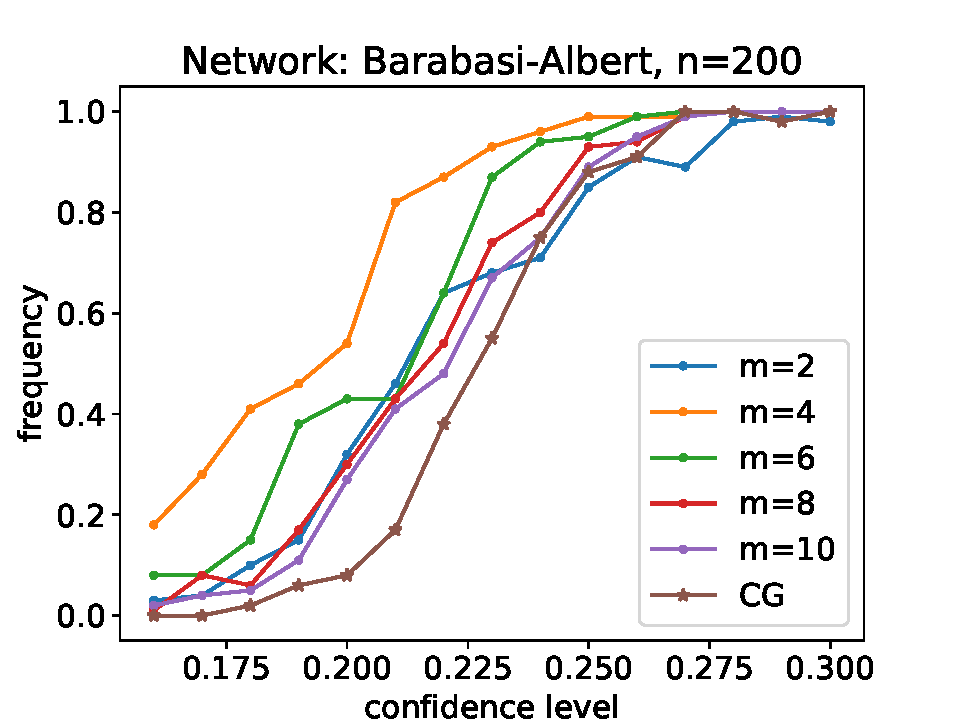
\includegraphics[width=\textwidth]{/home/arti/studia/python/praca_magisterska/plots/freq_consensus_ba_200.pdf}
		\caption{Frequency of reaching consensus for Barabasi--Albert network with $n=200$}
\end{figure}

We can observe that starting from $m=4$ and increasing it, we less often achieve consensus and the plot lines are closer to complete graph case. We may claim that the less connections the network has, the more eager it is to achieve consensus. This is not all the truth because for $m=2$ the network is weak--connected and consensus isn't established so often as there are not many links between agents. These results and results form Watts--Strogatz network case implies that networks for which agents don't have many connections are more eager to agree on consensus than well--connected networks. Of course, too weak--connected network does not establish consensus so often.

%\subsubsection{Comparison between networks}
%We would like also to compare a few weak--connected networks with each other and with complete graph to pick what are main differences in frequency of reaching consensus between them.

%\begin{figure}[H]
%		\centering
%		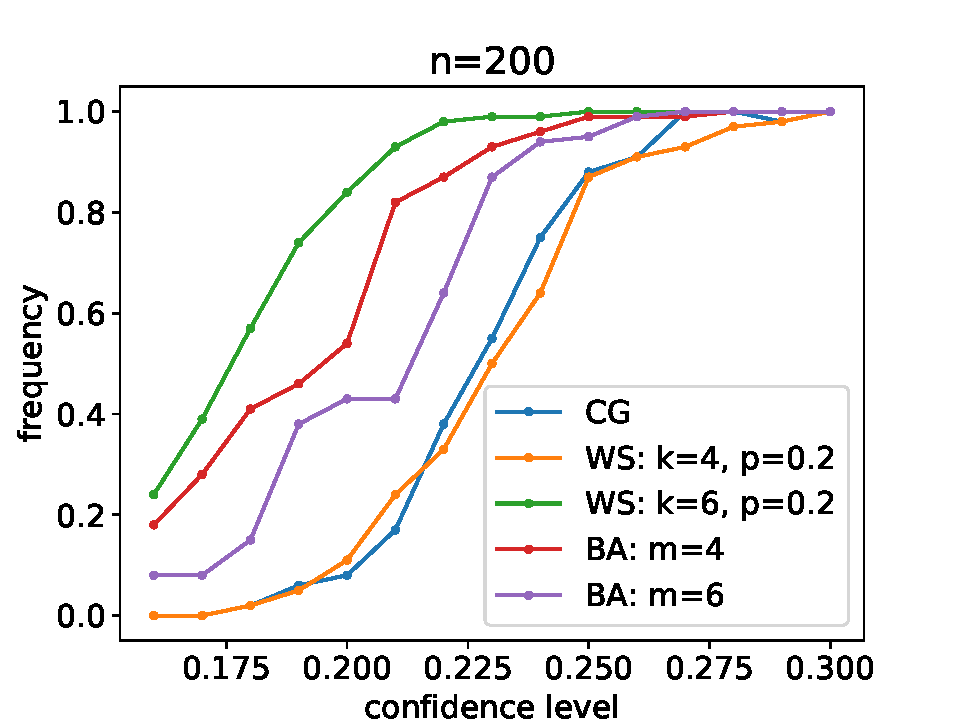
\includegraphics[width=\textwidth]{/home/arti/studia/python/praca_magisterska/plots/freq_consensus_compare.pdf}
%		\caption{Frequency of reaching consensus for various networks}
%\end{figure}



\subsection{Opinions changes through simulation}
In this section we will study average changes of agents opinions through opinions evolution process. We will investigate what is average change of opinions depending on confidence level, we will take into account final agents opinions and their initial ones and calculate average opinion change by the following formula:
\begin{equation}
\Delta x = \sum_{i=1}^n \left|x_{f}^{(i)} - x_0^{(i)} \right|,
\end{equation}
where $x_0^{(i)}$ is initial opinion of $i$-th agent and $x_{f}^{(i)}$ is his final opinion.

\indent

We will also study what is the dynamics of opinions changes depending on given network. In order to do this after each Monte Carlo step of Bounded Confidence model simulation, we calculate average value of opinion change, that is:
\begin{equation}
\Delta x_t = \sum_{i=1}^n \left|x_{t+1}^{(i)} - x_t^{(i)} \right|
\end{equation}



\subsubsection{Complete graph}

\begin{figure}[H]
		\centering
		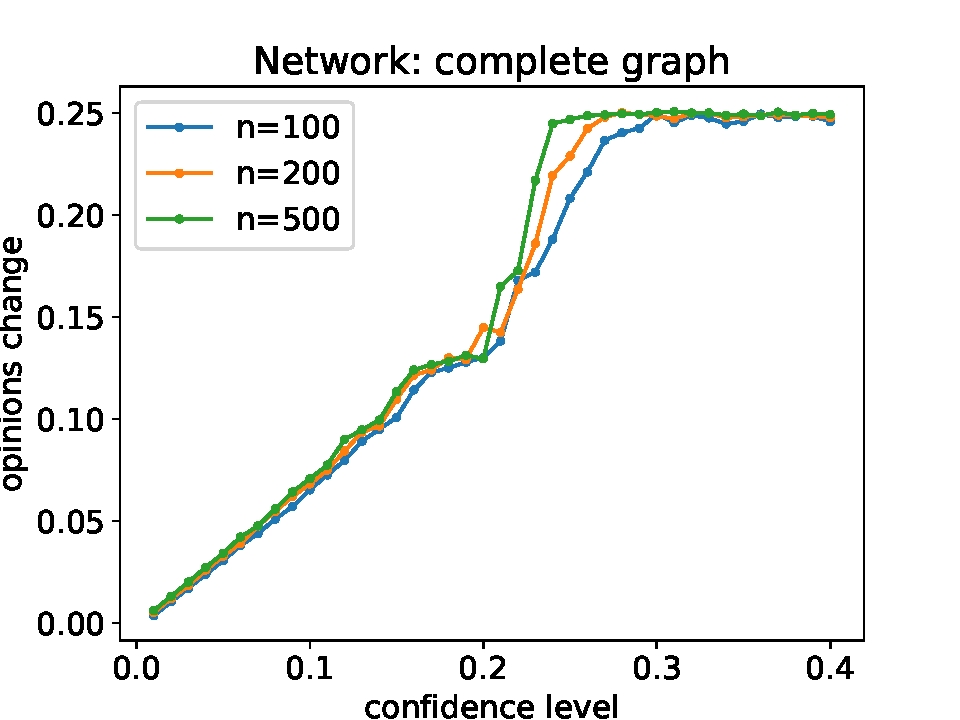
\includegraphics[width=\textwidth]{/home/arti/studia/python/praca_magisterska/plots/changes_completegraph.pdf}
		\caption{Average changes of opinions}
\end{figure}

We can see that bigger the value of confidence level is, average agents opinions change is also bigger. We observe linear growth up to confidence level $\epsilon=0.17$, at this point value of average opinions change is around $0.13$. Further on, up to $\epsilon=0.2$ opinions change increases only slightly, to this point plots for different network sizes are similiar. We may claim that $\epsilon=0.2$ is a breakpoint, because from that point small increase of confidence level causes significant increase of opinions change (especially for $n=500$). We also notify that the steepest growth is for biggest networks ($n=500$) and the mildest growth is for smallest networks ($n=100$). Finally, opinions changes stabilize on value $0.25$, which is typical case of consensus.

\indent

We already know how confidence level affects differences between initial agents opinions and final, but we would also like to know what is the dynamics of opinions changes.

\begin{figure}[H]
		\centering
		\includegraphics[width=\textwidth]{/home/arti/studia/python/praca_magisterska/plots/steps_changes_completegraph.pdf}
		\caption{Average changes of opinions in time space}
\end{figure}



\subsection{Fragmentation of opinions}

\section{Summary}
\indent

\end{document}